% 2026-10-22作者指示：本图改回单栏，按栏宽居中，保留全部原数据。
% cxy批注修改：按投稿清晰度要求适当放大密集图，使主要标注接近图题字号；原矢量内容与数据不变。
% 双Y轴组合图：按作者要求移除4条后保留30条线路；柱为相对CX时间降低率，线为Hellinger保真度。
% 横向参考线为30条线路的算术平均；不再绘制末尾Mean组。
% 单栏图：重新绘制为86×130 mm，参考示例加粗字体、合并图例、上下两图均显示倾斜线路标签；上下排列两种拓扑，图注同栏。
\begin{figure*}[!t]\centering
\setlength{\abovecaptionskip}{2pt}
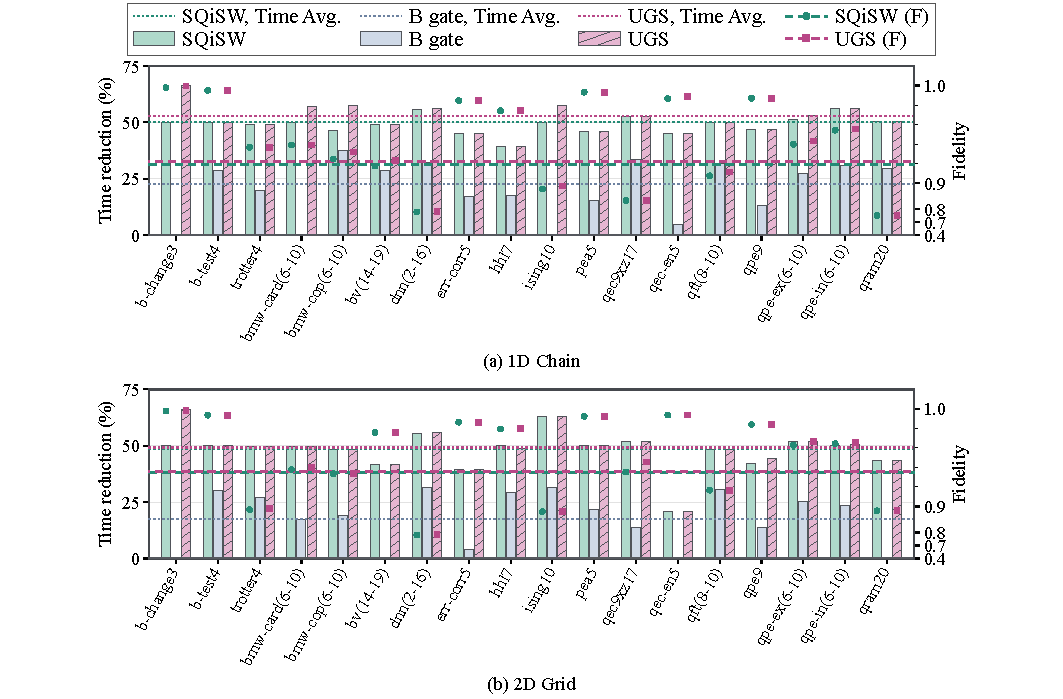
\includegraphics[width=\textwidth]{assets/fig13_restricted_topology_dual_axis.pdf}
\caption{Routed performance for 30 circuits on (a) 1D Chain and (b) 2D Grid.The fidelity axis uses a piecewise scale. }
\label{fig:12}
% 翻译：图12：在(a)一维链和(b)二维网格上的路由后性能。柱表示相对CX的时间降低率，图例中标F的点表示Hellinger保真度。每组对标签范围内实际测试的比特规模取平均。点状和虚线水平线分别为全部30条线路的时间与保真度均值，按组内线路数加权。负降低率在取均值后显示为0。保真度轴采用分段比例，压缩0.4至0.8并扩展0.9至1.0。
% 2026-10-22：图题与后续正文额外留8pt，避免视觉粘连。
\par\vspace{8pt}
\end{figure*}
